\documentclass[12pt,aspectratio=169]{beamer}

\usetheme{metropolis}

\definecolor{mDarkBrown}{HTML}{FF5722}
\definecolor{mDarkTeal}{HTML}{263238}
\definecolor{mLightBrown}{HTML}{FF5722}

\usepackage{booktabs}
\usepackage{graphicx}
\usepackage{hyphenat}
\usepackage{multirow}
\usepackage{nicefrac}
\usepackage[normalem]{ulem}

\usepackage[weather]{ifsym}

\usepackage{pifont}
\newcommand{\cmark}{\ding{51}}
\newcommand{\xmark}{\ding{55}}

\usepackage{minted}
\usemintedstyle{tango}
\newminted[bash]{bash}{%
    autogobble,
    bgcolor=mDarkTeal!10,
    linenos
}
\newminted[py3]{python}{%
    python3,
    autogobble,
    bgcolor=mDarkTeal!10,
    linenos
}
\newminted[sql]{sql}{%
    autogobble,
    bgcolor=mDarkTeal!10,
    linenos
}

\usepackage{polyglossia}
\setdefaultlanguage[variant=british]{english}
\usepackage[english=british]{csquotes}

\defaultfontfeatures{Ligatures=TeX}
\setmainfont{Lucida Sans OT}
\setsansfont[Scale=MatchLowercase]{Lucida Sans OT}
\setmonofont[Scale=MatchLowercase]{Lucida Console DK}

\usepackage{mathspec}
\setmathsfont(Digits,Latin,Greek)[Numbers={Lining,Proportional}]{Lucida Bright Math OT}

\newcommand{\mat}[1]{\ensuremath{\mathbf{#1}}}

\newcommand{\R}{\ensuremath{\mathbb{R}}}

\newcommand{\E}[1]{\ensuremath{\mathbb{E}\!\left[ #1 \right]}}
\newcommand{\V}[1]{\ensuremath{\mathbb{V}\!\left[ #1 \right]}}
\newcommand{\Prob}[1]{\ensuremath{\Pr\!\left( #1 \right)}}
\newcommand{\Normal}[2]{\ensuremath{\mathcal{N}\!\left( #1, #2 \right)}}
\newcommand{\simiid}{\ensuremath{\overset{\text{\tiny i.i.d.}}{\sim}}}

\DeclareMathOperator{\logit}{logit}

\author{Gianluca Campanella}
\date{}



\title{Introduction to neural networks}

\begin{document}

\maketitle

\begin{frame}{Perceptrons}
    \only<1>{%
        \begin{center}
            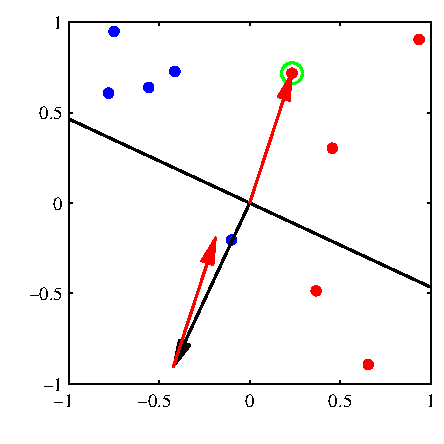
\includegraphics[height=0.8\textheight]{figures/perceptron_update_1} \\
            {\scriptsize%
             From \textit{Pattern Recognition and Machine Learning}}
        \end{center}}
    \only<2>{%
        \begin{center}
            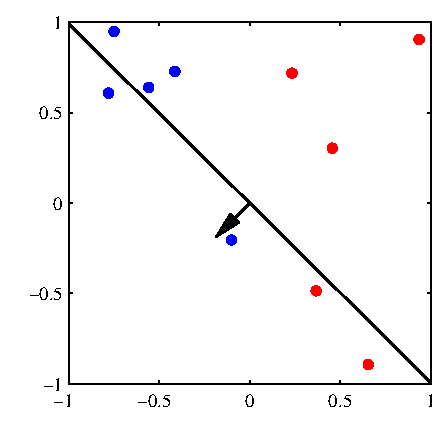
\includegraphics[height=0.8\textheight]{figures/perceptron_update_2} \\
            {\scriptsize%
             From \textit{Pattern Recognition and Machine Learning}}
        \end{center}}
    \only<3>{%
        \begin{center}
            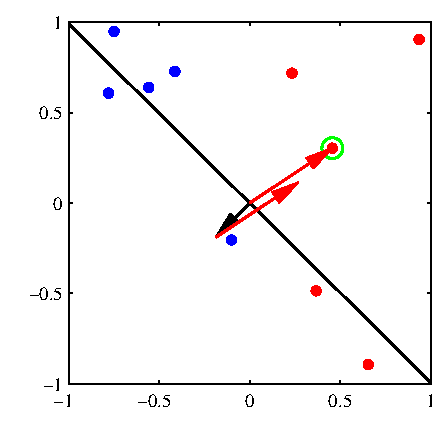
\includegraphics[height=0.8\textheight]{figures/perceptron_update_3} \\
            {\scriptsize%
             From \textit{Pattern Recognition and Machine Learning}}
        \end{center}}
    \only<4>{%
        \begin{center}
            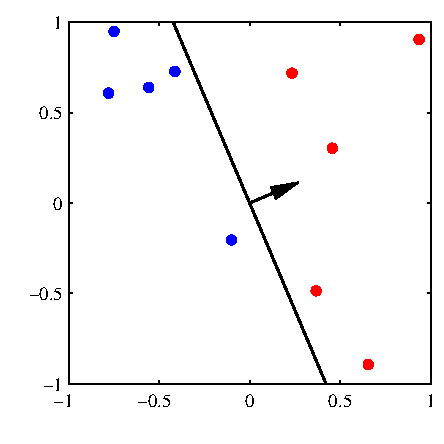
\includegraphics[height=0.8\textheight]{figures/perceptron_update_4} \\
            {\scriptsize%
             From \textit{Pattern Recognition and Machine Learning}}
        \end{center}}
    \only<5>{%
        \begin{block}{Support vector machines}
            \begin{itemize}
                \item Are trained on the entire dataset at once
                \item Try to find the largest possible margin
            \end{itemize}
        \end{block}
        \vfill
        \begin{block}{Perceptrons}
            \begin{itemize}
                \item Can be trained online (as the data arrives)
                \item Do not necessarily maximise the margin
            \end{itemize}
        \end{block}}
\end{frame}

\begin{frame}{Perceptrons and neurons}
    \only<1>{%
        \begin{center}
            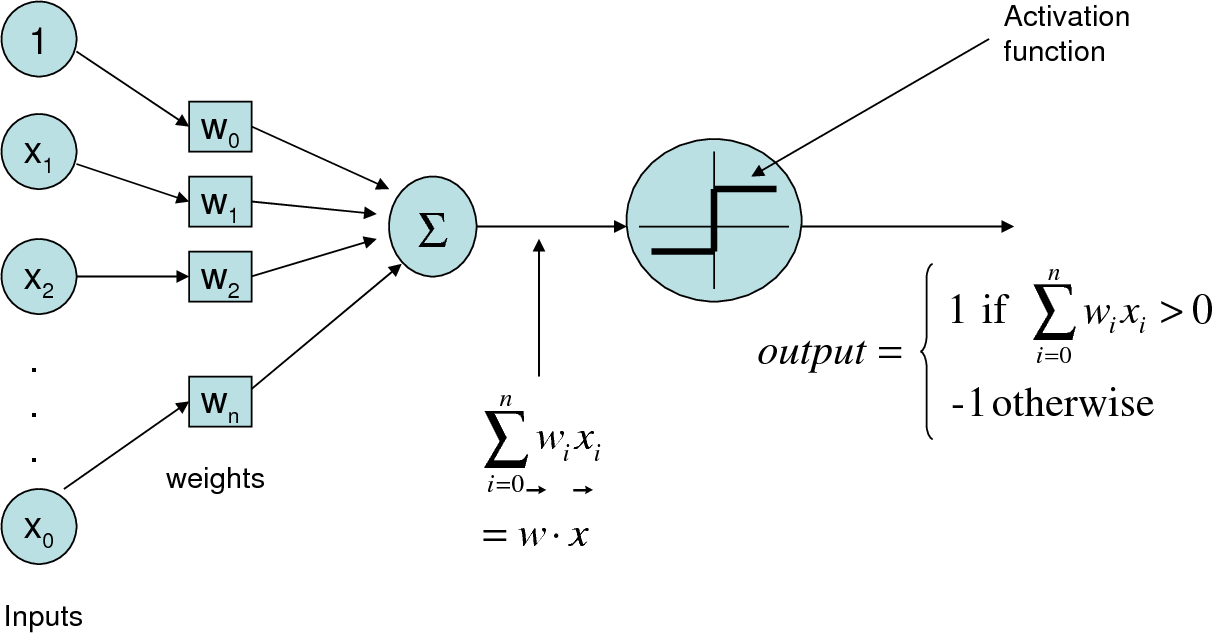
\includegraphics[height=0.8\textheight]{figures/perceptron} \\
            {\scriptsize%
             From Verma et al.\ (2015)}
        \end{center}}
\end{frame}

\begin{frame}{Multi\hyp{}layer perceptrons}
    \only<1>{%
        \begin{center}
            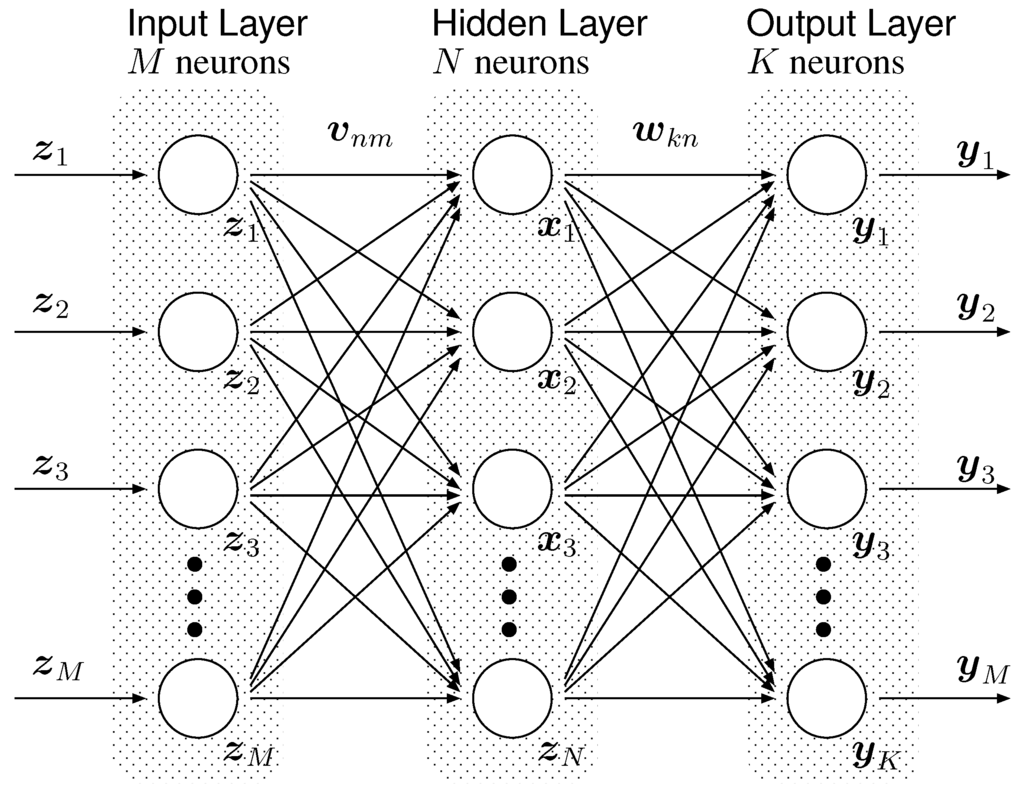
\includegraphics[height=0.85\textheight]{figures/mlp}
        \end{center}}
    \only<2>{%
        \begin{block}{Feed\hyp{}forward of information}
            \begin{itemize}
                \item Receive a new sample $X$ with outcome $y$
                \item Compute value for each unit in each layer
                \item Compute prediction $\hat{y}$ and error $\hat{\epsilon}$
            \end{itemize}
        \end{block}}
    \only<3>{%
        \begin{block}{Back\hyp{}propagation of error}
            \begin{itemize}
                \item Compute `blame'\ldots
                      \begin{itemize}
                          \item For output units: $y - \hat{y}$
                          \item For all other layers, as weighted contribution to
                                blame of following layer's units
                      \end{itemize}
                \item Adjust weights and biases
            \end{itemize}
        \end{block}}
    \only<4>{%
        \begin{block}{Questions}
            \begin{itemize}
                \item How many hidden layers?
                \item How many units in each layer?
                \item Which activation function?
                \item How do we initialise weights?
                \item How do we minimise error?
            \end{itemize}
        \end{block}}
\end{frame}

\begin{frame}{Other common topologies}
    \begin{block}{Convolutional neural networks}
        \begin{itemize}
            \item Inspired by the organisation of the visual cortex
            \item Include convolutional and pooling layers
        \end{itemize}
    \end{block}
    \vfill
    \begin{block}{Recurrent neural networks}
        \begin{itemize}
            \item Possess `internal memory'
            \item Can process sequences of inputs
        \end{itemize}
    \end{block}
\end{frame}

\begin{frame}{Pros and cons}
    \begin{block}{Pros}
        \begin{itemize}
            \item Can handle large datasets
            \item Effective in high\hyp{}dimensional spaces ($p > n$)
            \item Predictions are fast
        \end{itemize}
    \end{block}
    \vfill
    \begin{block}{Cons}
        \begin{itemize}
            \item Can require considerable parameter tuning
            \item Training is somewhat cumbersome
            \item New data can cause `forgetfulness'
        \end{itemize}
    \end{block}
\end{frame}

\end{document}

